\pagenumbering{roman}
%%%%%%%%%%%%%%%%%%%%%%%%%%%
% Diplomaterv-kiiras (ezt adjak, bele kell kötni a diplomába)
%%%%%%%%%%%%%%%%%%%%%%%%%%%
\begin{center}

\textbf{BUDAPEST UNIVERSITY OF TECHNOLOGY AND ECONOMICS}

\medskip


\includegraphics[width=8.79cm]{images/bme.pdf}

\medskip

\textbf{FACULTY OF ELECTRICAL ENGINEERING AND INFORMATICS\\SOFTWARE ENGINEERING}

 \vspace{2cm}
 \Large\textbf{\cim}

 \vspace{6mm}
 \textbf{\nev} \\
 \texttt{<vsza@vsza.hu>} \\ \strut \\

 \Large\textbf{THESIS STUDY}

\end{center}

\vfill

Consultant:

\begin{center}
\konzulens\\ \konzbeoszt

\vspace{96pt}

December 2011
\end{center}

% \vspace{6mm}
% \begin{tabular}{p{80mm}l}
% A záróvizsga tárgyai:   & Első tárgy \\
%                         & Második tárgy \\
%                         & Harmadik tárgy
%  \end{tabular}
%
%  \vspace{6mm}
%  \begin{tabular}{p{80mm}l}
%  A tervfeladat kiadásának napja:         &  \\
%  A tervfeladat beadásának határideje:    &
%  \end{tabular}
%
% \vfill
%
% \begin{center}
% \begin{tabular}{cc}
%  \makebox[7cm]{\emph{dr.\ Görgényi András}}    & \makebox[7cm]{\emph{dr.\ Péceli Gábor}} \\
%  \makebox[7cm]{adjunktus, diplomaterv felelős} & \makebox[7cm]{egyetemi tanár, tanszékvezető}
% \end{tabular}
% \end{center}
%
%  \vspace{6mm}
%  \begin{tabular}{p{80mm}l}
%  A tervet bevette:           & \\
%  A terv beadásának dátuma:   & \\
%  A terv bírálója:            &
%  \end{tabular}


 \thispagestyle{empty}
 \blankpage

\selectlanguage{magyar}
%%%%%%%%%%%%%%%%%%%%%%%%%%%
% Diplomaterv-kiiras melleklete (ezt is adjak, bele kell kötni a diplomába)
%%%%%%%%%%%%%%%%%%%%%%%%%%%
 \begin{textblock*}{\paperwidth}(0mm,0mm)
    \noindent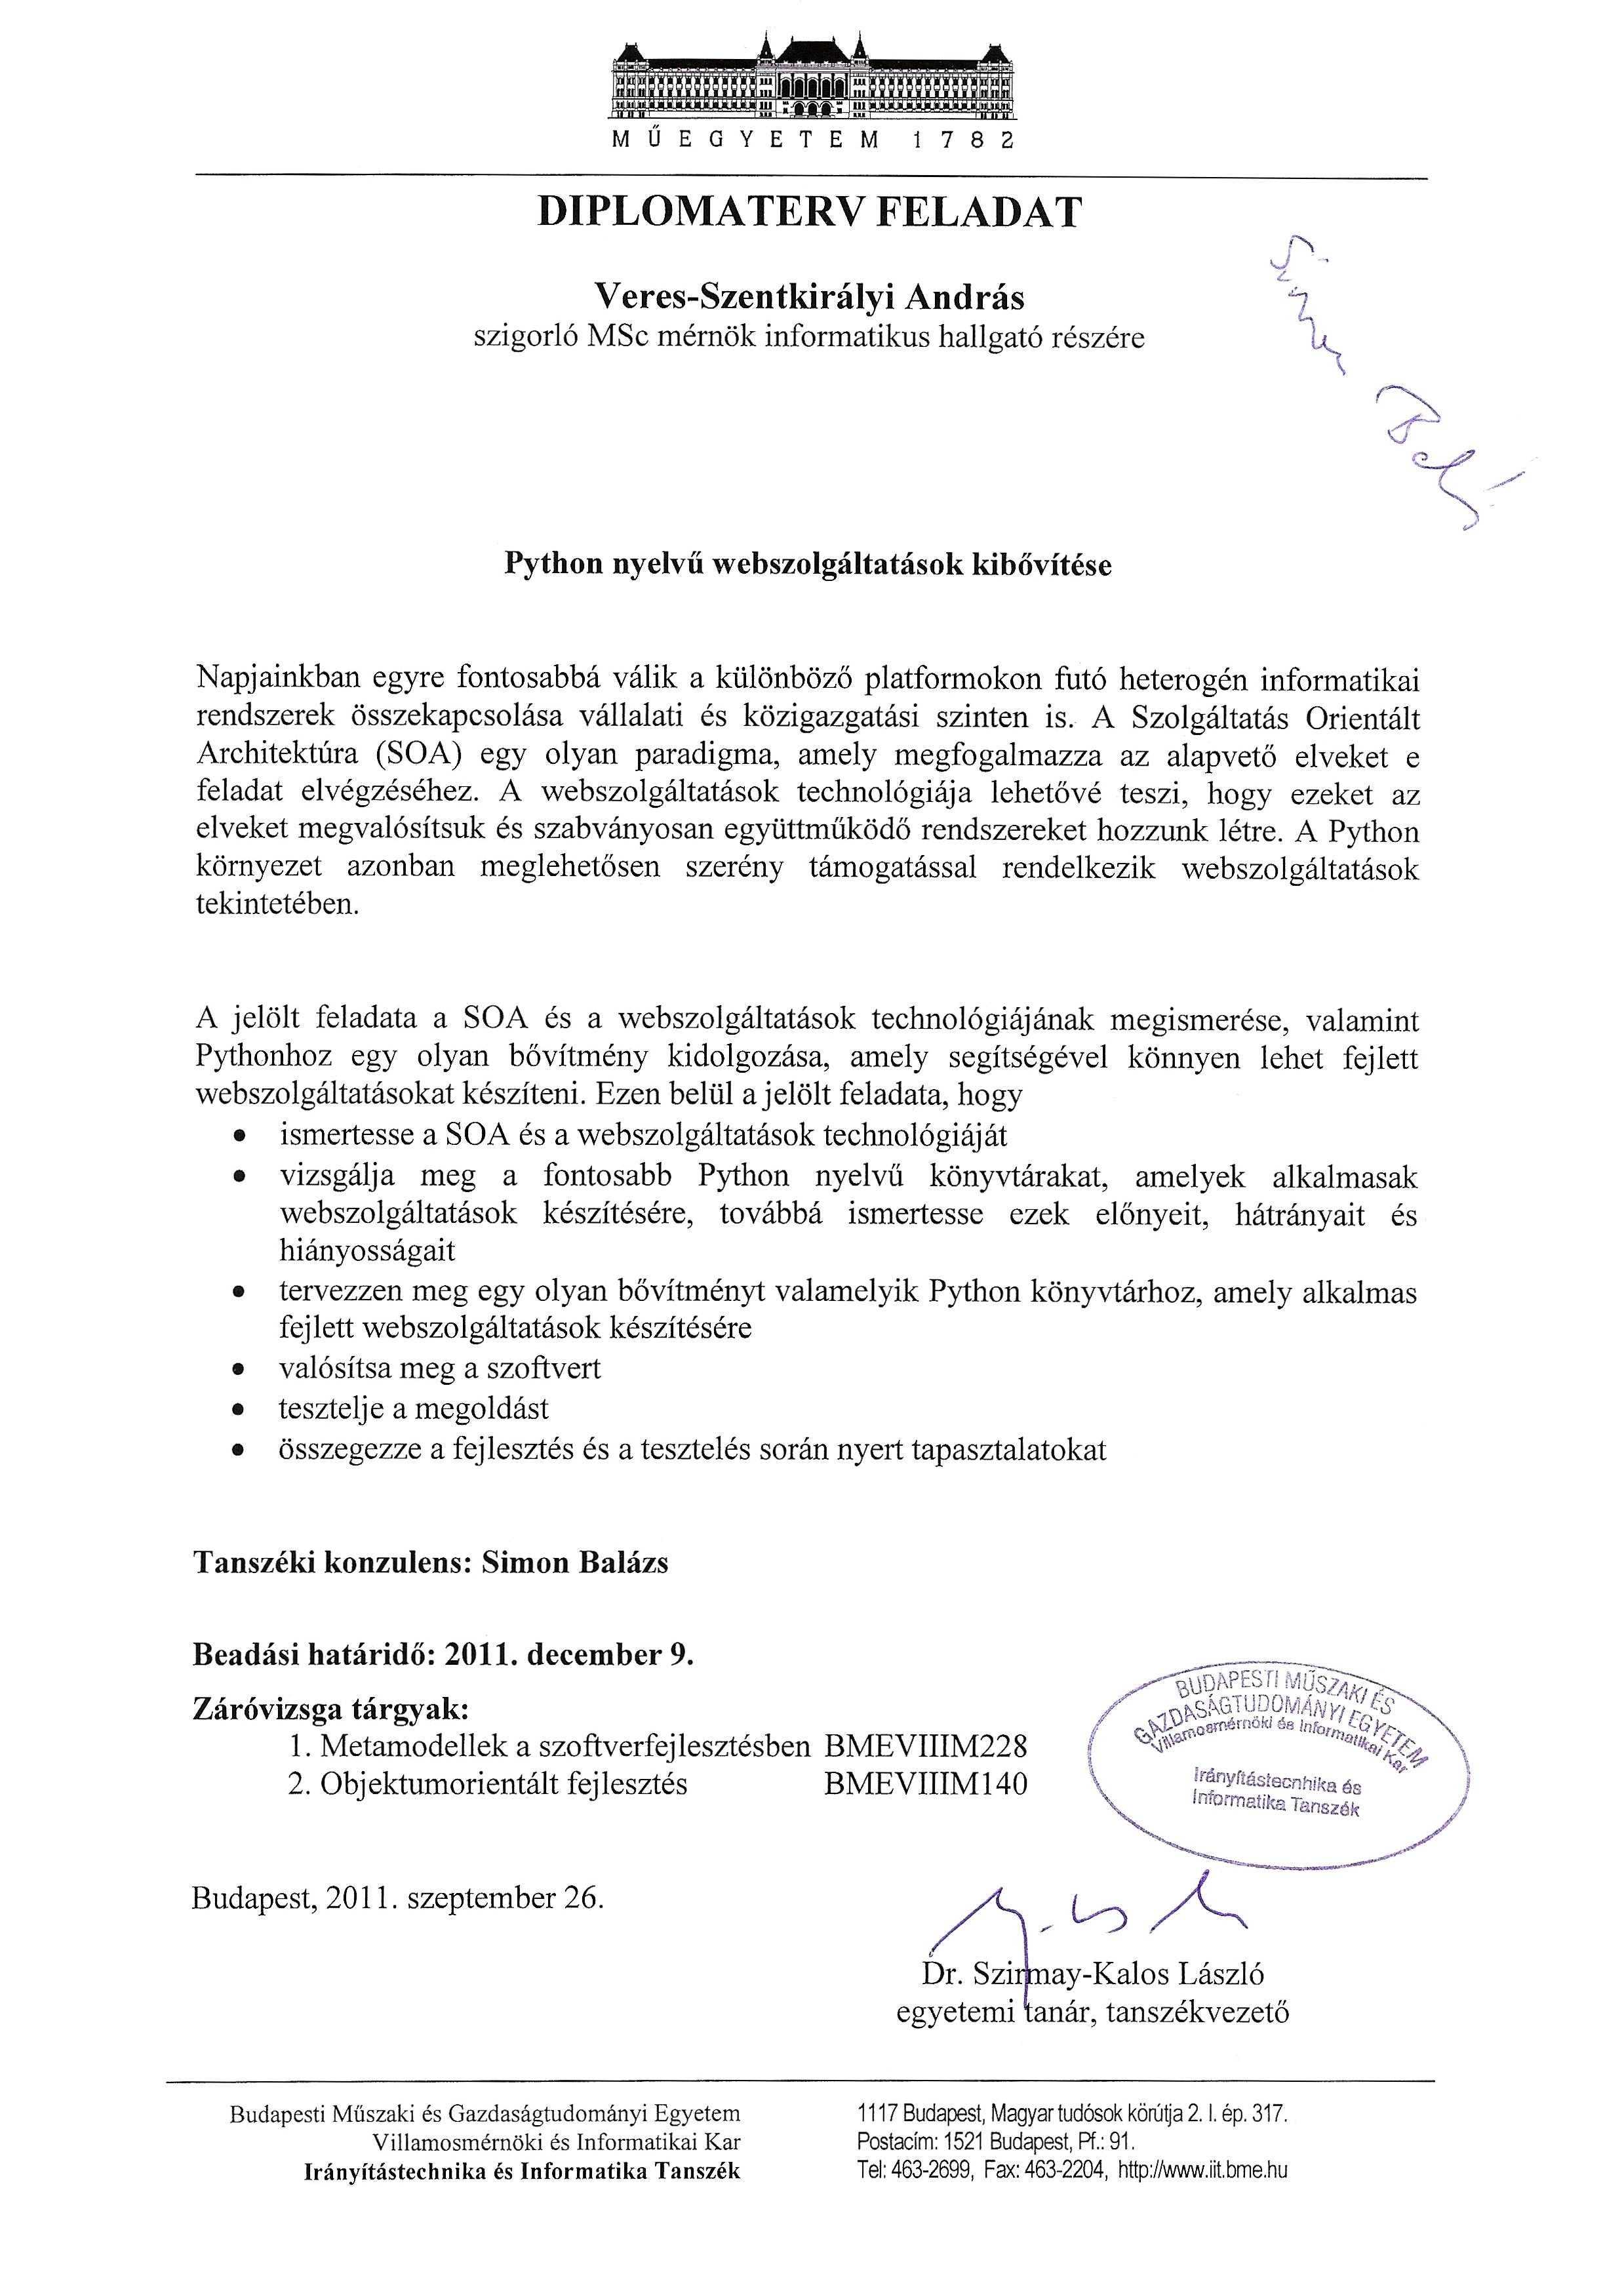
\includegraphics[width=\paperwidth,height=\paperheight]{images/feladat-retouched.jpg}
	\end{textblock*}
	\mbox{}
 \blankpage

%%%%%%%%%%%%%%%%%%%%%%%%%%%
% Nyilatkozat
%%%%%%%%%%%%%%%%%%%%%%%%%%%
\def\abstractname{Nyilatkozat}
\begin{abstract}

\noindent
Alulírott \emph{Veres-Szentkirályi András}, szigorló hallgató kijelentem,
hogy ezt a diplomatervet meg nem engedett segítség nélkül, saját  magam
készítettem, csak a megadott forrásokat (szakirodalom, eszközök, stb.)
használtam fel. Minden olyan  részt, amelyet szó szerint, vagy azonos
értelemben, de átfogalmazva más forrásból átvettem, egyértelműen, a
forrás megadásával megjelöltem.

Hozzájárulok, hogy a jelen munkám alapadatait (szerző(k), cím, angol és magyar
nyelvű tartalmi kivonat, készítés éve, konzulens(ek) neve) a BME VIK nyilvánosan
hozzáférhető elektronikus formában, a munka teljes szövegét pedig az egyetem
belső hálózatán keresztül (vagy autentikált felhasználók számára) közzétegye.
Kijelentem, hogy a benyújtott munka és annak elektronikus verziója megegyezik.
Dékáni engedéllyel titkosított diplomatervek esetén a dolgozat szövege csak 3 év
eltelte után válik hozzáférhetővé.
\begin{flushright}
 \vspace*{1cm}
 \makebox[7cm]{\rule{6cm}{.4pt}}\\
 \makebox[7cm]{\emph{Veres-Szentkirályi András}}\\
 \makebox[7cm]{hallgató}
\end{flushright}
\end{abstract}

%%%%%%%%%%%%%%%%%%%%%%%%%%%
% Tartalomjegyzek
%%%%%%%%%%%%%%%%%%%%%%%%%%%
\selectlanguage{english}
\tableofcontents

%%%%%%%%%%%%%%%%%%%%%%%%%%%
% Kivonat
%%%%%%%%%%%%%%%%%%%%%%%%%%%
\def\abstractname{Kivonat}
\selectlanguage{magyar}
\begin{abstract}
\addcontentsline{toc}{chapter}{Kivonat}
% TODO
\end{abstract}


%%%%%%%%%%%%%%%%%%%%%%%%%%%
% Abstract
%%%%%%%%%%%%%%%%%%%%%%%%%%%
\selectlanguage{english}
\begin{abstract}
\addcontentsline{toc}{chapter}{Abstract}
% TODO
\end{abstract}
